\section{Results}

\subsection{Experimental Overview}

The full experiment was conducted on 139 bug reports collected from the
Minecraft issue tracking dataset. Each report was independently annotated
using the proposed quality assessment framework and assigned a quality score
ranging from 1 to 5.

Two prompting strategies were evaluated:

\begin{itemize}
    \item Raw Prompt
    \item Improved Prompt
\end{itemize}

The outputs generated by the Large Language Model (LLM) were compared
against the human-annotated ground truth. Performance was evaluated using
Accuracy, Macro Precision, Macro Recall, Macro F1-score, and Cohen's Kappa.
In addition, confusion matrices and score distributions were analyzed to
provide further insights into the agreement patterns between the LLM and
human annotations.

\subsection{Raw Prompt Results}

Table~\ref{tab:raw_results} summarizes the performance obtained using the
Raw Prompt configuration.

\begin{table}[!t]
\centering
\caption{Performance Metrics for Raw Prompt}
\label{tab:raw_results}
\begin{tabular}{lc}
\toprule
Metric & Value \\
\midrule
Accuracy & 69.18\% \\
Precision (Macro) & 56.07\% \\
Recall (Macro) & 55.01\% \\
F1-score (Macro) & 53.22\% \\
Cohen's Kappa & 0.5776 \\
\bottomrule
\end{tabular}
\end{table}

The Raw Prompt configuration achieved moderate performance across all
evaluation metrics. The overall Accuracy reached 69.18\%, while the Macro
F1-score was 53.22\%, indicating that the model experienced difficulty in
maintaining consistent prediction quality across all score categories.

\begin{figure}[!t]
\centering
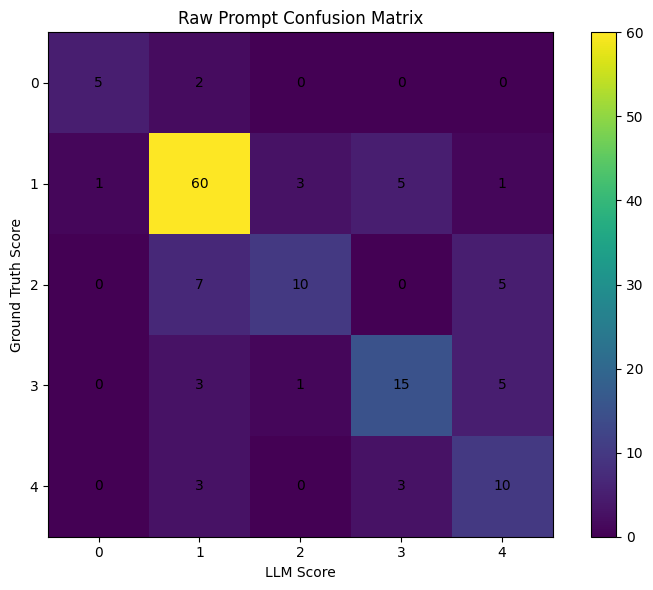
\includegraphics[width=\linewidth]{figures/raw_confusion_matrix.png}
\caption{Confusion Matrix for the Raw Prompt configuration.}
\label{fig:raw_matrix}
\end{figure}

Figure~\ref{fig:raw_matrix} illustrates the confusion matrix obtained using
the Raw Prompt strategy. The model correctly classified a large proportion
of reports assigned score 2 by human annotators. However, considerable
misclassification remained among the higher score categories, particularly
between scores 3, 4, and 5.

\begin{figure}[!t]
\centering
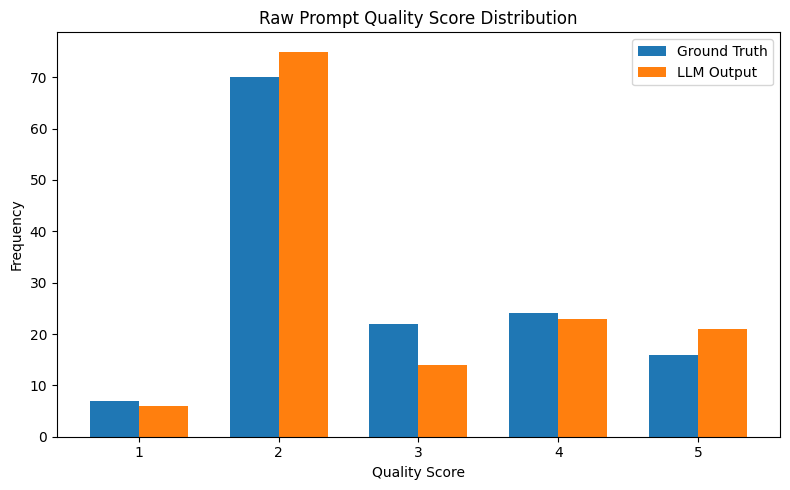
\includegraphics[width=\linewidth]{figures/raw_distribution.png}
\caption{Quality score distribution for the Raw Prompt configuration.}
\label{fig:raw_distribution}
\end{figure}

The score distribution shown in Figure~\ref{fig:raw_distribution}
demonstrates noticeable differences between the LLM-generated scores and
the human annotations. While the overall trend is similar, the Raw Prompt
configuration tends to overestimate some quality levels and underestimate
others, resulting in reduced agreement with the ground truth.

\subsection{Improved Prompt Results}

After refining the prompt design and introducing clearer evaluation
instructions, the model achieved improved performance across most metrics.

\begin{table}[!t]
\centering
\caption{Performance Metrics for Improved Prompt}
\label{tab:improved_results}
\begin{tabular}{lc}
\toprule
Metric & Value \\
\midrule
Accuracy & 76.26\% \\
Precision (Macro) & 57.09\% \\
Recall (Macro) & 55.58\% \\
F1-score (Macro) & 55.73\% \\
Cohen's Kappa & 0.3345 \\
\bottomrule
\end{tabular}
\end{table}

The Improved Prompt configuration achieved the highest overall Accuracy
(76.26\%) and Macro F1-score (55.73\%). These results indicate that prompt
engineering can positively influence the model's ability to assess bug
report quality.

\begin{figure}[!t]
\centering
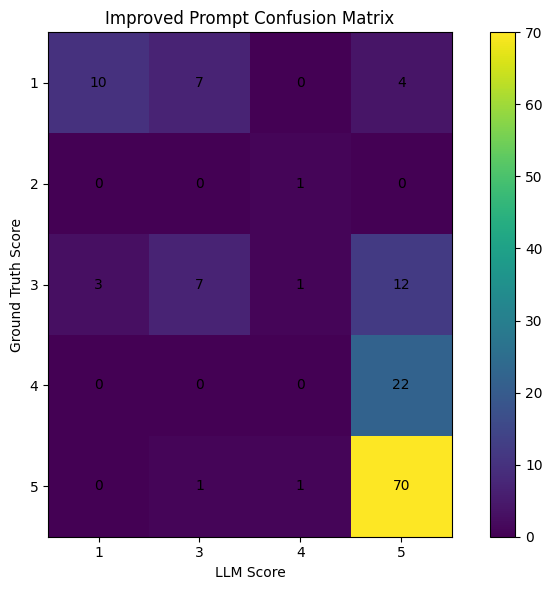
\includegraphics[width=\linewidth]{figures/improved_confusion_matrix.png}
\caption{Confusion Matrix for the Improved Prompt configuration.}
\label{fig:improved_matrix}
\end{figure}

Figure~\ref{fig:improved_matrix} shows that the Improved Prompt increased
the number of correctly predicted reports receiving the highest quality
score. Most reports rated highly by human annotators were also assigned
high scores by the LLM.

\begin{figure}[!t]
\centering
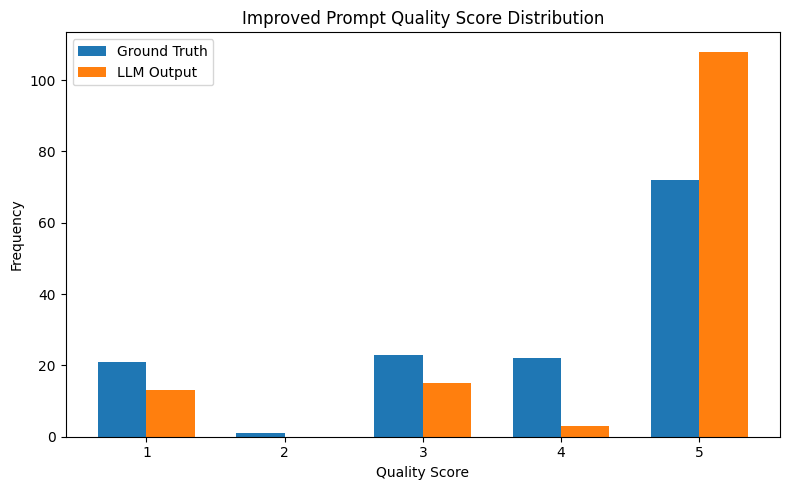
\includegraphics[width=\linewidth]{figures/improved_distribution.png}
\caption{Quality score distribution for the Improved Prompt configuration.}
\label{fig:improved_distribution}
\end{figure}

The distribution presented in Figure~\ref{fig:improved_distribution}
reveals a stronger concentration of predictions in the highest quality
category. Compared with the Raw Prompt, the Improved Prompt generated
outputs that more closely followed the overall pattern of the human
annotations.

\subsection{Comparison Between Prompt Configurations}

Table~\ref{tab:comparison} compares the performance of the two prompting
strategies.

\begin{table}[!t]
\centering
\caption{Comparison Between Raw and Improved Prompts}
\label{tab:comparison}
\begin{tabular}{lcc}
\toprule
Metric & Raw Prompt & Improved Prompt \\
\midrule
Accuracy & 69.18\% & 76.26\% \\
Precision (Macro) & 56.07\% & 57.09\% \\
Recall (Macro) & 55.01\% & 55.58\% \\
F1-score (Macro) & 53.22\% & 55.73\% \\
Cohen's Kappa & 0.5776 & 0.3345 \\
\bottomrule
\end{tabular}
\end{table}

The Improved Prompt outperformed the Raw Prompt on Accuracy, Precision,
Recall, and F1-score. Accuracy increased by approximately seven percentage
points, while the Macro F1-score improved from 53.22\% to 55.73\%.

Interestingly, Cohen's Kappa decreased from 0.5776 to 0.3345. This result
suggests that although the Improved Prompt produced more accurate
predictions overall, the score distribution became more concentrated in
certain categories, reducing agreement after correcting for chance.

\subsection{Distribution Analysis}

The confusion matrices and score distributions provide additional insight
into the behavior of the LLM. The Raw Prompt exhibited broader score
dispersion and more frequent confusion among neighboring categories. In
contrast, the Improved Prompt generated more consistent high-quality
predictions and reduced classification noise.

The distribution figures further indicate that prompt refinement helped the
model better recognize high-quality bug reports. However, the tendency to
assign high scores more frequently may also explain the reduction observed
in Cohen's Kappa.

\subsection{Summary of Findings}

The experimental results demonstrate that prompt engineering can improve
the performance of LLM-based bug report quality assessment. The Improved
Prompt achieved the highest Accuracy (76.26\%) and Macro F1-score
(55.73\%), indicating stronger alignment with human annotations.

Overall, the findings suggest that carefully designed prompts can enhance
the reliability of automated bug report evaluation, while also highlighting
the importance of considering both predictive performance and agreement
metrics when assessing LLM behavior.